% [原文 p.145]
\begin{equation}
  \begin{tikzpicture}[>=stealth, baseline=(current bounding box.center)]
    \node (A) at (2.0,1.5) {$K(X)$};
    \node (B) at (7.6,1.5) {$K_{S_k}(X^k)$};
    \node (C) at (7.6,-1.5) {$K_{S_k}(X)$};
    \draw[->] (A) -- node[above] {$\otimes^k$} (B);
    \draw[->] (B) -- node[right] {$d^*$} (C);
    \draw[->] (A) -- node[below, sloped, pos=0.58] {$\otimes^k$} (C);
  \end{tikzpicture}
  \tag{B.3.4}
\end{equation}
% 本图式承接 p.144 末句「次の可換図式が得られる」，原书编号为 (B.3.4)；p.145 顶部无其他正文。

\section{算子与滤过}
\takeaway{本节用限制映射 $K(X)\to K(X_{q-1})$ 的核给出 $K(X)$ 的滤过 $K_q(X)$，把“$x\in K_q\Rightarrow x^k\in K_{kq}$”推广为张量幂的滤过估计（定理 B.4.3、B.4.5），并算出 $B_{\Z/k}$ 上滤过的具体形式（引理 B.4.6）。}

从现在起，假定空间 $X,Y,\dots$ 都是有限 CW 复形。此时，由
\[
  K_q(X)=\Ker\{K(X)\to K(X_{q-1})\}
\]
定义的部分群 $K_q(X)$ 给出 $K(X)$ 的一个滤过；其中 $X_{q-1}$ 表示 $X$ 的 $(q-1)$ 骨架。于是 $K_0(X)=K(X)$；若 $\dim X<n$，则 $K_n(X)=0$。此外，如 [8] 所示，对一切 $q$ 都成立
\[
  K_{2q}(X)=K_{2q-1}(X).
\]
任意映射 $Y\to X$ 都与某个胞腔映射同伦，因此该滤过是自然的。

% [Tutor Note: “$q$ 切片”是日译本对骨架（skeleton）的译名，本书一律称“$q$ 骨架”。注意 $K_q(X)$ 由限制映射 $K(X)\to K(X_{q-1})$ 的核定义：$q$ 越大条件越强、$K_q$ 越小，故这是“余维 $\ge q$”型的滤过，与按骨架递增的拓扑滤过方向相反。]

论文 [8] 证明 $K(X)$ 是滤过环，即 $K_p(X)\cdot K_q(X)\subset K_{p+q}(X)$。特别地可知
\[
  x\in K_q(X)\Rightarrow x^k\in K_{kq}(X).
\]
试把这一结果推广到张量幂 $\otimes^k$。

首先回想：对任意有限群有自然同态
\[
  \alpha\colon R(G)\to K(B_G),
\]
其中 $B_G$ 是 $G$ 的分类空间 [5]。这个同态如下确定。

% [原文 p.146]
设 $A$ 为 $B_G$ 的万有覆盖，$V$ 为 $G$-模。此时 $A\times_G V$ 是 $B_G$ 上的向量丛。对应 $V\mapsto A\times_G V$ 诱导同态
\[
  \alpha\colon R(G)\to K(B_G).
\]
这一构造可以推广如下。设 $X$ 为 $G$ 空间，用 $X_G$ 记空间 $A\times_G X$。若 $V$ 是 $X$ 上的 $G$-向量丛，则
\[
  V_G=A\times_G V
\]
是 $X_G$ 上的向量丛。此时对应 $V\mapsto V_G$ 诱导同态
\[
  \alpha_X\colon K_G(X)\to K(X_G).
\]

这里需要几点说明。首先，为了统一 $B_G$ 与 $X_G$ 的记号用法，注意 $A\times_G\{*\}=B_G$，故不妨把 $B$ 看作表示单点集。其次，$B_G$ 与 $X_G$ 都不是有限复形。不过 $B_G$ 虽是无穷维复形，仍可使每个 $q$ 骨架 $B_{G,q}$ 都是有限复形，于是把 $K(B_G)$ 定义为
\[
  K(B_G)=\varinjlim_{q}K(B_{G,q}).
\]
假定 $G$ 在 $X$ 上的作用是胞腔的：取 $A_q$ 为 $B_{G,q}$ 的万有覆盖，令 $X_{G,q}=A_q\times_G X$，则 $X_{G,q}$ 是有限复形。此时定义
\[
  K(X_G)=\varinjlim_{q}K(X_{G,q}).
\]
后面会看到，实际上无须取极限：本文的结果本质上只涉及有限骨架。引入无穷复形 $B_G$、$X_G$，只是因为比起始终处理有限近似，这样看问题略微清楚一些。

% [Tutor Note: $K(B_G)$、$K(X_G)$ 的定义是沿骨架取正向极限，故 (B.4.1) 中出现的 $K(X\times B_{S_k})$ 实际应读作 $\varinjlim_q K(X\times B_{S_k,q})$；书中此后不再重复这层意思。]

把这些构造用于群 $S_k$ 与空间 $X$（平凡作用）或 $X^k$（轮换作用），便得到交换图式

% [原文 p.147]
\begin{equation}
  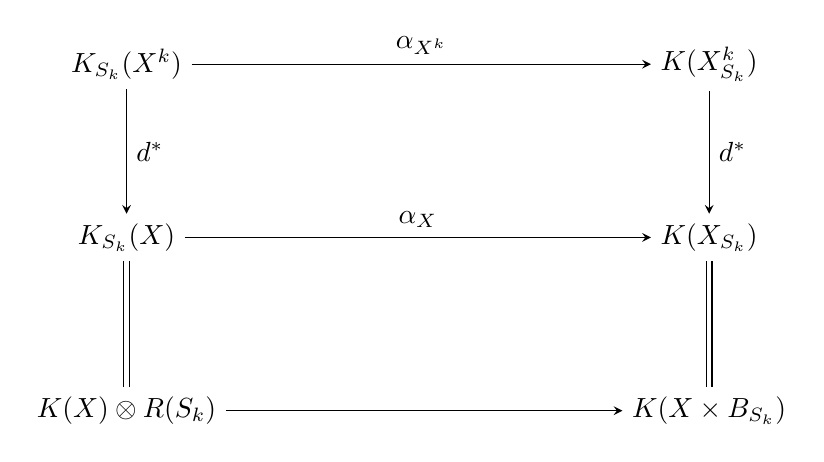
\begin{tikzpicture}[>=stealth, baseline=(current bounding box.center)]
    \node (A1) at (0,2.2) {$K_{S_k}(X^k)$};
    \node (B1) at (7.4,2.2) {$K(X^k_{S_k})$};
    \node (A2) at (0,0) {$K_{S_k}(X)$};
    \node (B2) at (7.4,0) {$K(X_{S_k})$};
    \node (A3) at (0,-2.2) {$K(X)\otimes R(S_k)$};
    \node (B3) at (7.4,-2.2) {$K(X\times B_{S_k})$};
    \draw[->] (A1) -- node[above] {$\alpha_{X^k}$} (B1);
    \draw[->] (A1) -- node[right] {$d^*$} (A2);
    \draw[->] (A2) -- node[above] {$\alpha_X$} (B2);
    \draw[->] (B1) -- node[right] {$d^*$} (B2);
    \draw[double, double distance=1.6pt] (A2) -- (A3);
    \draw[double, double distance=1.6pt] (B2) -- (B3);
    \draw[->] (A3) -- (B3);
  \end{tikzpicture}
  \tag{B.4.1}
\end{equation}
其中 $d^*$ 表示由对角映射 $d\colon X\to X^k$ 诱导的映射。

\begin{proposition*}{B.4.2}
  设 $x\in K_q(X)$。则
  \[
    \alpha_{X^k}(x^{\otimes k})\in K_{kq}(X^k_{S_k}).
  \]
\end{proposition*}

\begin{proof}
  由假设，$x$ 含于
  \[
    K(X)\to K(X_{q-1})
  \]
  的核中。于是取 $Y=X_{q-1}$ 应用推论 B.3.3，可知 $x^{\otimes k}$ 含于下面图式中 $\rho$ 的核内：
  \begin{equation*}
    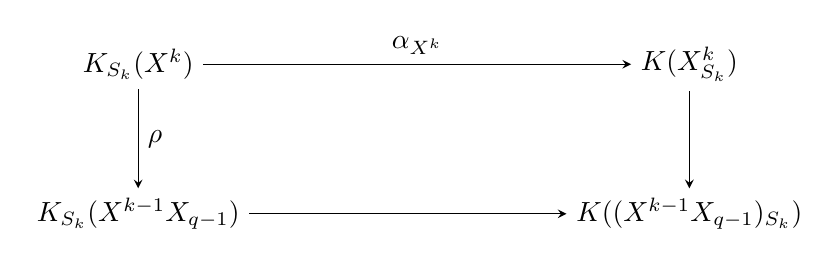
\begin{tikzpicture}[>=stealth, baseline=(current bounding box.center)]
      \node (A1) at (0,1.9) {$K_{S_k}(X^k)$};
      \node (B1) at (7.0,1.9) {$K(X^k_{S_k})$};
      \node (A2) at (0,0) {$K_{S_k}(X^{k-1}X_{q-1})$};
      \node (B2) at (7.0,0) {$K((X^{k-1}X_{q-1})_{S_k})$};
      \draw[->] (A1) -- node[above] {$\alpha_{X^k}$} (B1);
      \draw[->] (A1) -- node[right] {$\rho$} (A2);
      \draw[->] (B1) -- (B2);
      \draw[->] (A2) -- (B2);
    \end{tikzpicture}
  \end{equation*}
  这样一来，只须验证
  \[
    (X^k_{S_k})_{kq-1}\subset (X^{k-1}X_{q-1})_{S_k},
  \]
  所求结论便由该图式得出。现在，$X^k_{S_k}=X^k\times_{S_k}A$ 的 $(kq-1)$ 骨架的任意胞腔 $\sigma$ 都是 $X$ 的 $k$ 个胞腔与 $A$ 的一个胞腔之积。于是 $X$ 的这 $k$ 个胞腔中至少有一个维数小于 $q$，从而 $\sigma$ 含于

  % [原文 p.148]
  \[
    (X^{k-1}X_{q-1})_{S_k}=X^{k-1}X_{q-1}\times_{S_k}A
  \]
  之中，即所求。
\end{proof}

% [Tutor Note: 证明中 $X^{k-1}X_{q-1}$ 是简写，指乘积空间 $X^{k-1}\times X_{q-1}$；$A$ 即 $B_{S_k}$ 的万有覆盖。]

由于 $K$ 群上的滤过是自然的，把命题 B.4.2 与图式 (B.4.1)、推论 B.3.3 合起来，便得到下面的主要结果。

\begin{theorem}{B.4.3}
  设 $\otimes k\colon K(X)\to K(X)\otimes R(S_k)$ 为张量幂算子，
  \[
    \alpha\colon K(X)\otimes R(S_k)\to K(X\times B_{S_k})
  \]
  为自然同态。此时
  \[
    x\in K_q(X)\Rightarrow\alpha(x^{\otimes k})\in K_{kq}(X\times B_{S_k})
  \]
  成立。
\end{theorem}

\begin{corollary*}{B.4.4}
  设 $\dim X\le n$ 且 $x\in K_q(X)$。则 $x^{\otimes k}$ 在 $K(X)\otimes K(B_{S_k,kq-n-1})$ 中的像为零。
\end{corollary*}

\begin{proof}
  由定理 B.4.3，$x^{\otimes k}$ 在 $K(X\times B_{S_k,kq-n-1})$ 中的像为零。然而对任意空间 $A,B$，映射
  \[
    K(A)\otimes K(B)\to K(A\times B)
  \]
  都是单射 [6]。因此 $x^{\otimes k}$ 在 $K(X)\otimes K(B_{S_k,kq-n-1})$ 中的像为零，即推论所述。
\end{proof}

\begin{remark}{}
  由定理 B.4.3，对任意有限群 $G$ 与 $G$ 空间 $X$，$K_G(X)$ 的滤过应当定义为
  \[
    K_G(X)_q=\alpha_X^{-1}K_q(X\times B_G).
  \]
  采用这一记法，定理 B.4.3 就可以简单地写成

  % [原文 p.149]
  \[
    x\in K_q(X)\Rightarrow x^{\otimes k}\in K_{S_k}(X)_{kq}
  \]
  的形式。
\end{remark}

为了使用定理 B.4.3，必须清楚地了解 $K(B_{S_k})$ 的滤过；这由下面的定理给出。

\begin{theorem*}{B.4.5}
  假定 $K(X)$ 无挠，且 $\dim X\le n$。设 $x\in K_q(X)$，并假定对一切 $i,j>0$、$i+j\le k$，乘积 $\lambda^i(X)\lambda^j(x)$ 都为零。此时取命题 B.2.4 中的 $M$，令 $m$ 是使
  \[
    m\alpha\lambda_{-1}(M)\in K_{kq-n}(B_{S_k})
  \]
  成立的最小整数，则 $\lambda^k(X)$ 被 $m$ 整除。特别地，在稳定范围 $n<2q$ 内上述结论成立。
\end{theorem*}

% [Tutor Note: 原书 p.149 此处印作 $\lambda^i(X)\lambda^j(x)$ 与 $\lambda^k(X)$，但同一页的证明随即写作 $\lambda^k(x)$，且 $\lambda$ 运算作用在 $K$ 群元素上，故疑为笔误，应读作 $\lambda^i(x)\lambda^j(x)$ 与 $\lambda^k(x)$。]

\begin{proof}
  由假设与命题 B.2.4 可导出
  \[
    x^{\otimes k}=(-1)^{k-1}\lambda^k(x)\otimes\lambda_{-1}(M)\in K(X)\otimes R(S_k).
  \]
  令 $A=K(B_{S_k})/K_{kq-n}(B_{S_k})$，则 $A$ 是 $K(B_{S_k,kq-n-1})$ 的子群。由推论 B.4.4 与 $K(X)$ 自由，$x^{\otimes k}$ 在 $K(X)\otimes A$ 中的像必须为零。因此 $\lambda^k(x)$ 被 $\lambda_{-1}(M)$ 在 $A$ 中的像的阶，亦即满足
  \[
    m\alpha\lambda_{-1}(M)\in K_{kq-n}(B_{S_k})
  \]
  的最小整数 $m$ 整除。
\end{proof}

\begin{remark}{}
  在命题 B.1.9 的证明中已经知道，$\lambda_{-1}(M)$ 的特征标在 $S_k$ 的所有阶为合数的轮换置换上为零。因此，若 $k$ 不是素数幂，则 $\lambda_{-1}(M)$ 的特征标在阶为素数幂的 $S_k$ 的所有元素上为零；由 [5, (6.10)]，$\lambda_{-1}(M)$ 含于同态
  \[
    R(S_k)\to\widehat{R(S_k)}
  \]
  的核中。于是 $\alpha\lambda_{-1}(M)=0$，定理 B.4.5 成为自明。所以定理 B.4.5 只在 $k$ 为素数幂时才有意义。
\end{remark}

% [原文 p.150]
为得到具体结果，需要把 $S_k$ 限制为循环群 $\Z/k$。此时计算是简单的。先需要下面的引理。

\begin{lemma*}{B.4.6}
  设 $Y=B_{\Z/k}$。则
  \[
    K(Y_{2q-1})\cong R(\Z/k)/I(\Z/k)^q
  \]
  成立。
\end{lemma*}

\begin{proof}
  $Y$ 的奇次整系数上同调为零，故可导出 $K^1(Y,Y_{2q-1})=0$；于是由这一对的完全列得到
  \[
    K(Y_{2q-1})\cong K(Y)/K_{2q}(Y).
  \]
  另一方面，已知
  \[
    K(Y)\cong\widehat{R(\Z/k)}
  \]
  （见 [5, (8.1)]），并且 $K_{2q}(Y)$ 是由 $I(\Z/k)^q$ 生成的理想。因此
  \[
    K(Y)/K_{2q}(Y)\cong R(\Z/k)/I(\Z/k)^q,
  \]
  引理得证。
\end{proof}

% [Tutor Note: $\widehat{R(\Z/k)}$ 表示表示环 $R(\Z/k)$ 对 $I(\Z/k)$-进拓扑的完备化；$I(\Z/k)$ 由增广理想（即 $R$ 中维数部分为零的元素）生成，$I(\Z/k)^q$ 是它的 $q$ 次幂。]

\begin{remark}{}
  从论文 [5] 引用的结果极其简单，把那里所用的计算直接用于 $Y_{2q-1}$ 也很容易。
\end{remark}

把推论 B.4.4 与引理 B.4.6 组合起来，便得到下面的命题。

\begin{proposition}{B.4.7}
  设 $\dim X\le 2m$，$x\in K_{2q}(X)$。此时 $k$ 次循环幂 $P^k(x)\in K(X)\otimes R(\Z/k)$ 含于 $K(X)\otimes I(\Z/k)^{kq-m}$ 的像中。
\end{proposition}

$k=p$ 为素数的情形特别有意义，因为此时 $\Z/p$ 是 $S_p$ 的 $p$-Sylow 子群。这意味着，就 $p$ 群的结果而言，从 $S_p$ 转到 $\Z/p$ 不会丢失任何东西。因此下一节详细考察 $\Z/p$ 的情形。

% [原文 p.151]
\section{素数阶循环群的情形}
\takeaway{本节把 $S_k$ 换成 $\Z/p$，在完备化 $\widehat{R(\Z/p)}$ 中把正则表示 $N$ 的幂按 $\eta=\rho-1$ 的幂次展开（引理 B.5.1、推论 B.5.2），据此得到 $\theta^p(x)$ 与 $\psi^p(x)$ 被 $p$ 的幂整除的定量结论（定理 B.5.3、推论 B.5.4）。}

\begin{lemma*}{B.5.1}
  用 $\rho\in R(\Z/p)$ 表示 $\Z/p$ 的一维标准表示，令
  \[
    N=\sum_{i=0}^{p-1}\rho^i
  \]
  为正则表示，并令 $\eta=\rho-1$。此时在 $\widehat{R(\Z/p)}$ 中有
  \[
    p^k(N-p)=(-1)^k\eta^{(k+1)(p-1)}+\text{高次项}.
  \]
\end{lemma*}

\begin{proof}
  由 $\rho^p=1$ 得 $(1+\eta)^p=1$。于是 $\eta^p=-p\eta\epsilon$，其中 $\epsilon\equiv1\bmod\eta$，从而是 $\widehat{R(\Z/p)}$ 的单位。因此，当存在满足 $\epsilon\equiv1\bmod\eta$ 的 $\epsilon$ 使 $a=\epsilon b$ 时记作 $a\sim b$，便有
  \begin{equation}
    (-p)\eta\sim\eta^p. \tag{1}
  \end{equation}
  这里，把等式
  \[
    \sum_{i=0}^{p-1}(1+t)^i=\frac{(1+t)^p-1}{t}\equiv p+t^{p-1}\bmod pt
  \]
  中的 $t$ 换成 $\eta$，利用 (1) 即可证明
  \begin{align*}
    N-p&\equiv\eta^{p-1}\bmod p\eta\\
    &\equiv\eta^{p-1}\bmod\eta^p.
  \end{align*}
  因此得到
  \begin{equation}
    (N-p)\sim\eta^{p-1}. \tag{2}
  \end{equation}
  由 (1) 又得到
  \[
    (-p)^k\eta\sim\eta^{k(p-1)}\eta,
  \]
  从而

  % [原文 p.152]
  \begin{equation}
    (-p)^k\eta^{p-1}\sim\eta^{(k+1)(p-1)} \tag{3}
  \end{equation}
  成立。至此，由 (2) 与 (3) 便推出本引理。
\end{proof}

\begin{corollary*}{B.5.2}
  $(N-p)$ 在 $R(\Z/p)/I(\Z/p)^n$ 中的像的阶为 $p^k$，其中 $k$ 是满足 $k+1\ge\frac{n}{p-1}$ 的最小整数。
\end{corollary*}

\begin{proof}
  $I(\Z/p)$ 是理想 $(\eta)$。
\end{proof}

% [Tutor Note: 推论 B.5.2 的 $k$ 由 $k+1\ge n/(p-1)$ 的最小整解决定，故 $k=\lceil n/(p-1)\rceil-1$；它与定理 B.5.3 证明中出现的 $k$ 是同一个量，注意两处下标不要混。]

至此可以陈述素数阶情形的具体结果。

\begin{theorem*}{B.5.3}
  设对 $t<q(p-1)$ 有 $\dim X\le2(q+t)$，并设 $x\in K_{2q}(X)$。此时令
  \[
    r=\left[\frac{t}{p-1}\right],
  \]
  则 $\theta^p(x)$ 被 $p^{q-r-1}$ 整除。
\end{theorem*}

\begin{proof}
  由 $\dim X<2qp$ 得 $x^p=0$。因此由命题 B.2.5，
  \[
    P^p(x)=\theta^p(x)\otimes(N-p)\in K(X)\otimes R(\Z/p).
  \]
  由命题 B.4.7，令 $n=pq-q-t$，则 $\theta^p(x)$ 被 $(N-p)$ 在 $R(\Z/p)/I(\Z/p)^n$ 中的像的阶整除。再由推论 B.5.2 可知 $\theta^p(x)$ 被 $p^k$ 整除，其中 $k$ 是满足
  \[
    (k+1)\ge q-\frac{t}{p-1}
  \]
  的最小整数，即
  \[
    k=q-\left[\frac{t}{p-1}\right]-1.
  \]
\end{proof}

\begin{corollary*}{B.5.4}
  与定理 B.5.3 作同样的假设。此时令 $r=\left[\frac{t}{p-1}\right]$，则 $\psi^p(x)$ 被 $p^{q-r}$ 整除。
\end{corollary*}

% [原文 p.153]
\begin{proof}
  $\psi^p$ 与 $\theta^p$ 满足关系式
  \[
    \psi^p(x)=x^p-p\theta^p(x).
  \]
  在目前的情形下 $x^p=0$，故
  \[
    \psi^p(x)=-p\theta^p(x),
  \]
  于是由系 B.5.2 立刻得到本系的结果。
\end{proof}
% [Tutor Note: 原书 p.153 此处引“系 B.5.2”，但 $\theta^p(x)$ 的可除性估计实际来自定理 B.5.3；系 B.5.2 只给出像的阶为 $p^k$。照原书抄录，此处的引用宜读作定理 B.5.3。]

\begin{remark}{}
  取 $t=0$，则当 $X=S^{2q}$ 为球面时，可知 $\psi^p(x)$ 被 $p^q$ 整除。应当注意，这一结果在书中并没有被明确用到任何地方。这个结果当然是周期性定理的推论，而对 $K(B_{\Z/p})$ 所用的计算当然也依赖于周期性定理。
\end{remark}

到此为止的结果，在 $X$ 无挠时特别有意义。先需要下面的引理。

\begin{lemma*}{B.5.5}
  假定 $X$ 无挠（即 $H^*(X;\Z)$ 无挠），设 $x\in K(X)$。假定 $x$ 在 $K(X_q)$ 中的像被 $d$ 整除。此时 $x$ 模 $K_{q+1}(X)$ 被 $d$ 整除，即
  \[
    x=dy+z,\quad y\in K(X),\ z\in K_{q+1}(X).
  \]
\end{lemma*}

\begin{proof}
  用 $A$ 与 $B$ 分别表示
  \[
    j^*\colon K(X)\to K(X_q)
  \]
  的像与余核。由对 $(X,X_q)$ 的完全列可知，$B$ 同构于 $K^1(X,X_q)$ 的一个子群。又因 $X$ 无挠，$X/X_q$ 也无挠，故 $K^1(X,X_q)$ 自由，从而 $B$ 自由。于是，若 $a\in A$ 在 $K(X_q)$ 中被 $d$ 整除，则 $a$ 在 $A$ 中也被 $d$ 整除。因此令 $a=j^*(x)$，则存在 $y\in K(X)$ 使

  % [原文 p.154]
  \[
    j^*(x)=dj^*(y),
  \]
  从而存在 $z\in\Ker j^*=K_{q+1}(X)$ 使 $x=dy+z$。
\end{proof}

由这一引理与推论 B.5.4 得到下面的命题。

\begin{proposition*}{B.5.6}
  假定 $X$ 无挠，设 $x\in K_{2q}(X)$。此时存在元素
  \[
    x_i\in K_{2q+2i(p-1)}(X)\quad(i=0,1,\dots,q),
  \]
  使
  \[
    \psi^p(x)=\sum_{i=0}^{q}p^{q-i}x_i;
  \]
  并且可以取 $x_q=x^p$。
\end{proposition*}

\begin{proof}
  令 $t=i(p-1)-1$。由定理 B.5.3，把 $\psi^p(x)$ 限制到 $2(q+t)$ 骨架上时，它被 $p^{q-i+1}$ 整除；由系 B.5.4 可导出 $\psi^p(x)$ 模 $K_{2q+2i(p-1)}(X)$ 被 $p^{q-i+1}$ 整除。于是所求结果可由对 $i$ 的归纳得到。由于 $\psi^p(x)\equiv x^p\bmod p$ 且 $x^p\in K_{2pq}(X)$，故可以取 $x_q=x^p$。
\end{proof}

% [Tutor Note: $\theta^p(x)$ 是 $P^p(x)=\theta^p(x)\otimes(N-p)$ 中的因子，$\psi^p$ 是 Adams 算子，二者由 $\psi^p(x)=x^p-p\theta^p(x)$ 相联系；命题 B.5.6 把 $\psi^p(x)$ 按 $p$ 的幂次展开，正是后面比较 Steenrod 作用素的入口。]

命题 B.5.6 中出现的元素 $x_i$ 并不由 $x$ 唯一确定。然而，转到伴随的分次群 $GK^*(X)$ 并模 $p$ 考虑时，由 $x_i$ 定义的元素
\[
  \overline{x_i}\in G^{2q+2i(p-1)}K(X)\otimes\Z/p
\]
由关系
\[
  \psi^p(x)=\sum_{i=0}^{q}p^{q-i}x_i
\]
唯一确定。把 $x$ 乘以 $p$，或者加上 $K_{2(q+1)}(X)$ 的任意元素，由引理 B.5.5 可知 $\overline{x_i}$ 都不改变。因此，$\overline{x_i}$ 只依赖于

% 块尾跨页句：よって，x̄_i は，…（原文 p.155 首行公式 $\overline{x_i}\in G^{2q}K(X)\otimes\Z/p$ 与「だけに依存する．」由 appB4 续完）
% CHUNK appB3 DONE
